\secnumbersection{MARCO CONCEPTUAL}

\subsection{PATHFINDING}

\textit{Pathfinding} es la creación de un plan de acción para cursar la ruta mas corta entre dos puntos, usando computación. El exponente inicial para la solución de este problema es el algoritmo de \textit{Dijkstra's} que encuentra la ruta optima en un grafo con costos en sus arcos desde un nodo a todos los otros.

En el trabajo con videojuegos se acostumbra a usar estos \textit{benchmarks} estandarizados \cite{sturtevant2012benchmarks}, estos han sido extraídos de juegos o creados para poner a prueba las distintas formas de encontrar la solución.

Es un punto importante del trabajo en videojuegos por la demanda de eficiencia, el trabajo desarrollado para el \textit{pathfinding} regularmente tiene un tiempo alocado que no permite buscar indefinidamente los caminos por lo cual es necesario tener medidas que han ido cambiando con los años para obtener resultados en el tiempo esperado, muchas veces esto genera agentes que se mueven de maneras innaturales pero entregarle mas tiempo a esto no es posible porque afectaría el desempeño del juego.

Normalmente se tienen que mover varios agentes en tiempo real y para esto existen distintos algoritmos. Antes de entrar a hablar de los distintos algoritmos, veremos un poco de la historia y teoría ocupada.

\subsection{TEORIA DE GRAFOS}

\subsubsection{DEFINICION DE GRAFO}

Un grafo G consiste en un grupo no vació, finito de nodos, $V(G)$, y un grupo finito de arcos de pares de nodos, $E(G)$. Un vértice \{v,w\}, uno los vértices $v$ y $w$. Se abrevia $vw$.

Los grafos que consideraremos serán mas simples porque no consideran mas de un arco entre los mismos dos nodos y no tienen arcos de un nodo a si mismo

La Figura \ref{fig:graph} muestra el grafo $G$, donde $V(G) = \{u,v,w,z\}$ y $E(G) = \{uv,uw,vw,wz\}$

\begin{figure}[h]
\centering
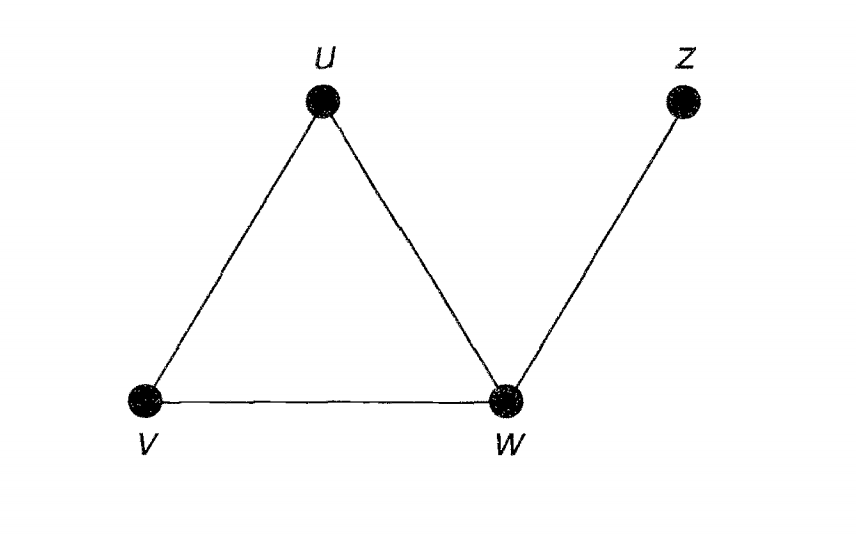
\includegraphics[width=0.5\textwidth]{grafo}
\caption{\label{fig:graph} Ejemplo de Grafo} Fuente: \textit{Introduction to Graph Theory} \cite{wilson1970introduction}.
\end{figure}

\subsubsection{CAMINO}

Un camino en un grafo $G$ es una secuencia finita de de arcos denotado por $v_o \rightarrow v_1 \rightarrow v_2 \rightarrow v_3 \rightarrow v_4 \rightarrow v_5...$

La Figura \ref{fig:graph2} muestra el grafo $G$, donde $V(G) = \{x,v,w,y,z\}$ y $E(G) = \{vx,vw,vy,wx$ $,wy,yx,xz,yz,zz\}$. Se pueden generar distintos caminos entre $v$ y $z$, de distintos largos, por ejemplo:

\begin{itemize}
\item $v \rightarrow w \rightarrow x \rightarrow z$ con largo 3.
\item $v \rightarrow y \rightarrow z$ con largo 2.
\end{itemize}

\begin{figure}[h]
\centering
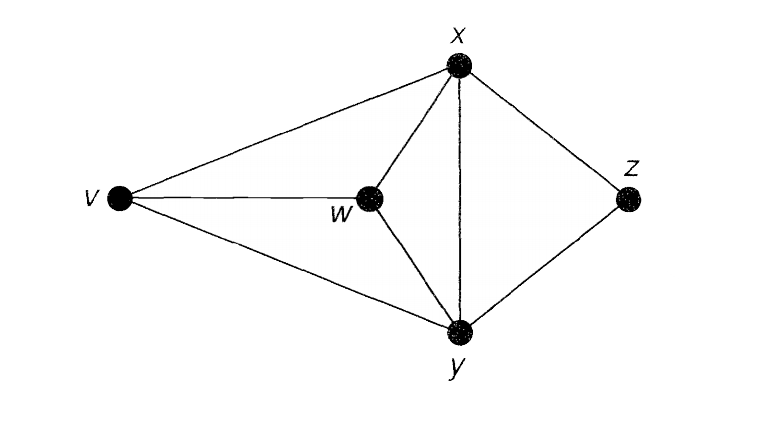
\includegraphics[width=0.5\textwidth]{grafo2}
\caption{\label{fig:graph2} Ejemplo de Camino en un Grafo} Fuente: Introduction to Graph Theory \cite{wilson1970introduction}.
\end{figure}

\subsubsection{COSTO}

Los arcos de los grafos que ocuparemos tendrán asociados un valor que llamaremos costo, donde el arco entre v y w se representa $\{v,w,X\}$ con $X \in \mathcal{R}^+ $

La Figura \ref{fig:graph3} muestra el mismo grafo anterior con valores en los arcos y compararemos los caminos mostrados antes, ahora con el costo total asociado.

\begin{itemize}
\item $v \rightarrow w \rightarrow x \rightarrow z$ con costo 3.
\item $v \rightarrow y \rightarrow z$ con costo 5.
\end{itemize}

En estos caminos podemos observar que el camino con menos arcos, no es mejor y esto es interesante cuando empezamos a trabajar en \textit{pathfinding}.

\begin{figure}[h]
\centering
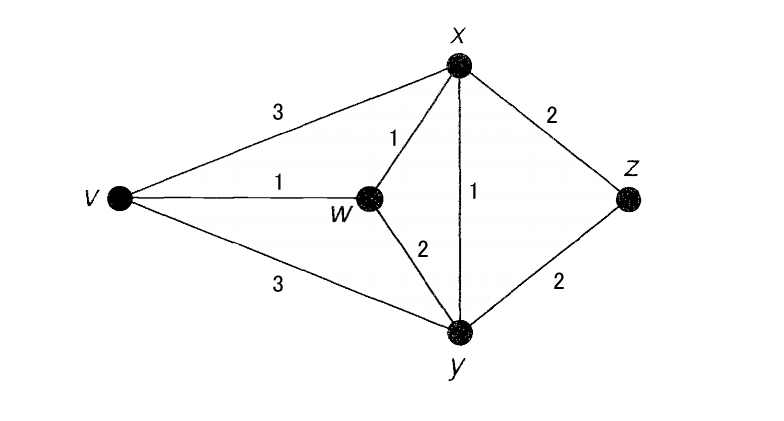
\includegraphics[width=0.5\textwidth]{grafo3}
\caption{\label{fig:graph3} Ejemplo de Camino en un Grafo con Costo en sus arcos} Fuente: \textit{Introduction to Graph Theory} \cite{wilson1970introduction}, con edición propia.
\end{figure}

\subsection{ALGORITMOS}

Los métodos de \textit{pathfinding}, comúnmente necesitan tres cosas. Un grafo para representar el mapa, un algoritmo de búsqueda y una heuristica para guiar la búsqueda.\cite{botea2013pathfinding}

Una forma muy común de representar los mapas, es en casillas como el ajedrez, que se consideran de forma atómica\footnote{El movimiento hacia dentro y fuera de la casilla se considera una acción por la búsqueda, no hay movimientos mas pequeños.}. Esta representación como grafo te permite aplicar el algoritmo de búsqueda.

Un primer acercamiento a un algoritmo para buscar un camino optimo es probar con todos los posibles caminos, esto se podría lograr con una búsqueda en profundidad. Pero se pueden eliminar caminos imposibles con anterioridad, o buscar en caminos mas problemas antes, por lo cual se usan heuristicas para acelerar la búsqueda.

Ahora entramos a hablar mas en detalle de los distintos algoritmos y heuristicas comúnmente ocupados para este problema.

\subsubsection{DIJKSTRA'S}

El algoritmo de \textit{Dijkstra's} \cite{dijkstra1959note} encuentra el camino mas corto entre dos nodos. Empieza con el nodo inicial y sus vecinos en un conjunto de opciones, en cada iteraccion selecciona el nodo con la menor distancia al inicial del conjunto de opciones, este queda marcado como visitado y sus vecinos que no han sido visitados entran al conjunto de opciones. Se repite este proceso hasta encontrar el nodo final o que este vacio el conjunto de opciones, en tal caso no existe un camino entre los nodos.

La primera version entregaba la distancia del camino, pero posteriores iteraciones han entregado el camino a todos los otros nodos desde el inicial o el camino a un nodo especifico entregado.
\newline

\begin{figure}[h]
\centering
\begin{lstlisting}[frame=single]
function Dijkstra(Graph, source):
    for each vertex v in Graph:      	// Inicializar
        dist[v] := infinity             //Dist. Desconocida
        previous[v] := undefined        // Nodo desconocido
    dist[source] := 0 	                // Nodo inicial
    Q := the set of all nodes in Graph 	// Nodos a recorrer
    while Q is not empty:               // Main loop
        u := node in Q with smallest dist[ ]
        remove u from Q
        for each neighbor v of u:       // Vecinos faltantes
            alt := dist[u] + dist_between(u, v)
            if alt < dist[v]            // Usar Dist. menor
                dist[v] := alt
                previous[v] := u
    return previous[ ]
\end{lstlisting}
\caption{\label{fig:dijisCode} Pseudo Codigo de algoritmo de \textit{Dijstra's}} Fuente: GITTA \cite{Brilliant2009April}.
\end{figure}


La Figura \ref{fig:djis} se muestra un grafo al que se le aplica este algoritmo para encontrar todos los caminos mínimos a el resto de sus nodos.


\begin{figure}[h]
\begin{minipage}[c]{0.5\textwidth}
	\centering
    Antes de la Búsqueda
	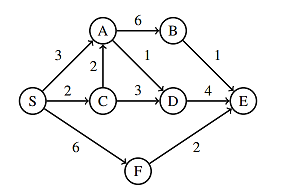
\includegraphics[width=1\textwidth]{djis1}
\end{minipage}
\begin{minipage}[c]{0.5\textwidth}
	\centering
    Después de la Búsqueda
	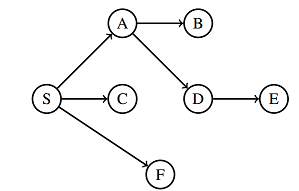
\includegraphics[width=1\textwidth]{djis2}
\end{minipage}
\caption{\label{fig:djis} Ejemplo de la aplicacion del algoritmo de Djkstra's} \begin{center}
	Fuente: \textit{Dijkstra's Shortest Path Algorithm} \cite{Brilliant2009April}.
\end{center}
\end{figure}

Cabe destacar que el algoritmo de \textit{Dijstra's} no funciona si existen arcos con costos negativos, pero esto no afecto a la búsqueda de caminos porque no tendría sentido que el agente se demorara un tiempo negativo en una acción.


\subsubsection{A*}

A* es una variación de \textit{Dijkstra's}, usa una heuristica que permite moverse a los nodos que están en dirección al objetivo. Logra esto sumando el peso del arco con una suposición de la distancia del nodo siguiente al nodo objetivo.

Esta suposición de la distancia es la heuristica, esta permite que no se revisen caminos posiblemente mas largos cuando existe la posibilidad de que exista un camino directo. 

El Seudo Codigo de A* es similar a Dijkstra's, el cambio a destacar es la diferencia que genera la heuristica(Como se ve en la figura \ref{fig:ACode}), en el ejemplo posterior estamos usando:

\begin{align*}
	heuristic(v,f) &= |v.x - f.x| + |v.y - f.y| \\
	v &= vertice\  actual \\
	f &= vertice\ final \\
	t.x &= posicion\ x\ en\ el\ tablero\ de\ vertice\ t \\
	t.y &= posicion\ y\ en\ el\ tablero\ de\ vertice\ t 
\end{align*}

	



\begin{figure}
\centering
\begin{lstlisting}[frame=single]
function A*(Graph, source, heuristic):
    for each vertex v in Graph:      	// Inicializar
        dist[v] := infinity             //Dist. Desconocida
        previous[v] := undefined        // Nodo desconocido
    dist[source] := 0 	                // Nodo inicial
    Q := the set of all nodes in Graph 	// Nodos a recorrer
    while Q is not empty:               // Main loop
        u := node in Q with smallest dist[ ]
        remove u from Q
        for each neighbor v of u:       // Vecinos faltantes
            alt := dist[u] + dist_between(u, v) + heuristic(v)
            if alt < dist[v]            // Usar Dist. menor
                dist[v] := alt
                previous[v] := u
    return previous[ ]
\end{lstlisting}
\caption{\label{fig:ACode} Pseudo Codigo de algoritmo \textit{A*}} Fuente: \textit{Introduction to A*} \cite{Red2016June}.
\end{figure}


Se ve en la figura \ref{fig:A}, el numero sobre las celdas muestra el valor con el que se toma la decisión de movimiento, como A* intenta usar el camino mas directo va directo a la muralla pero aun con esto explora menos que Dijkstra's que explora todo el tablero.

Aquí se ve como el uso de heuristicas puede mejorar la magnitud de la búsqueda necesaria para encontrar el camino optimo.

\begin{figure}
\begin{minipage}[c]{0.5\textwidth}
	\centering
    Antes de la Búsqueda
	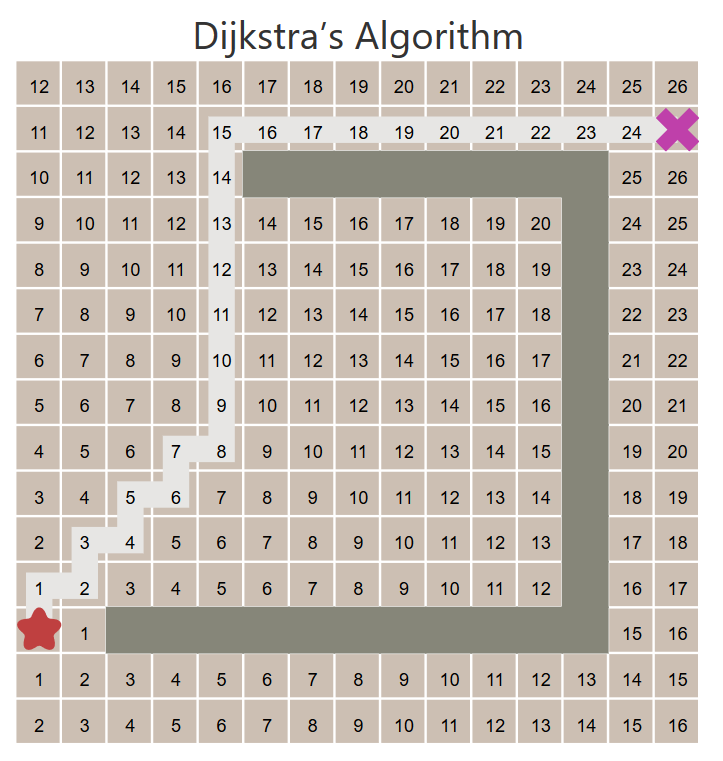
\includegraphics[width=1\textwidth]{djis3}
\end{minipage}
\begin{minipage}[c]{0.5\textwidth}
	\centering
    Después de la Búsqueda
	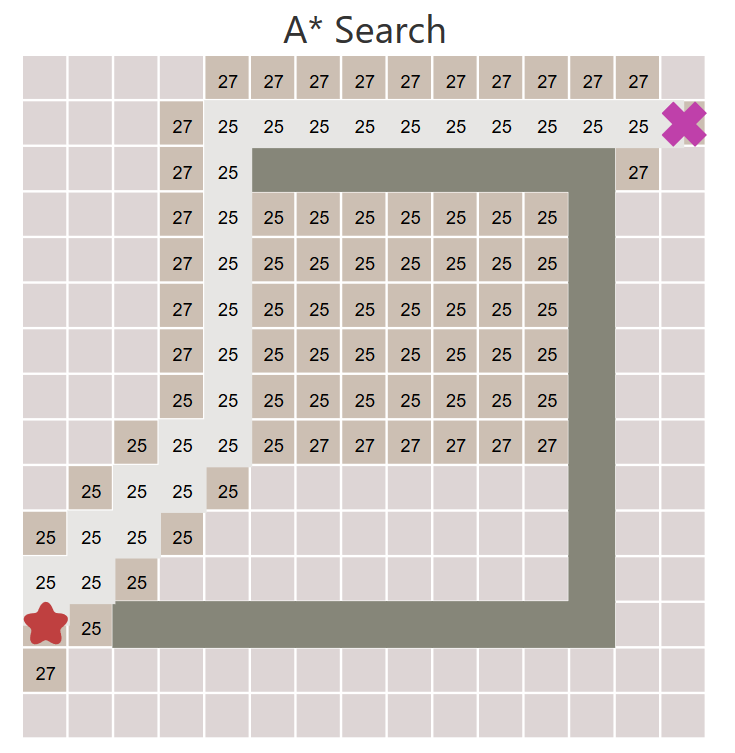
\includegraphics[width=1\textwidth]{A}
\end{minipage}
\begin{center}
\caption{\label{fig:A} Comparacion entre Dijkstra's y A*} 
Fuente: \textit{Introduction to A*}\cite{Red2016June}.
\end{center}
\end{figure}


\subsubsection{HEUTISTICAS}


Como vimos en A* usar heuristicas puede acelerar la búsqueda del camino, algunos ejemplos usados en la literatura son los siguientes.

\begin{enumerate}

\item \textit{Manhattan}: Explicada en la sección de A*. 

\item \textit{Octile}: Para los mapas que permiten movimiento diagonal, se usa con A* en estos mapas.

\begin{align*}
	Octile &= \sqrt{2}*m + (M-m) \\
	m &= min( \Delta x, \Delta y) \\
	M &= max( \Delta x, \Delta y)
\end{align*}

\item \textit{Differential}: \cite{goldberg2005computing}
 Se hace un paso de procesamiento previo calculando la distancia real desde todos los puntos a unas \textit{landmarks}\footnote{Puntos "importante" dentro del mapa, pueden ser cuellos de botella, posiciones predefinidas u otros}. Con esta información puedes calcular la heuristica para tener una estimación de la distancia entre el nodo $n_1$ y $n_2$ con todas las \textit{landmarks} L.

\begin{align*}
	Differential &= max(| d(n_1,l) - d(n_2,l) |),  \ l \in L \\
	d(n_x,l) &= distancia\ entre\ n_x\ y\ l
\end{align*}

Esto aproxima con la máxima distancia para evitar casos como que un \textit{landmark} este en medio de ambos nodos.

\item \textit{Dead-end}: \cite{bjornsson2006improved} Identifica areas que no tienen la solucion y les da un valor infinito. 
	
\item \textit{Gateway, canonical y portal}: \cite{bjornsson2006improved,sturtevant2009memory,goldenberg2010portal} Tres heuristicas que intentan separar el mapa en los cuellos de botella y precomputar movimientos entre los sectores creador

\end{enumerate}


\subsubsection{ABSTRACCIONES DE MAPA}







Como vimos, lo normal es representar el mapa en un tablero, existen algoritmos que toman este tablero y hacen abstracciones posteriores para encontrar soluciones de mayor nivel rápidamente, esto permite trabajar en grafos mas pequeños y después cortar el grafo original para buscar una solución. También permite tener una dirección aproximada mas rápidamente, lo cual puede permitir que el agente empiece su movimiento sin tener la solución completa.

Se tiene que tener claro que al encontrar una solución a un nivel mas alto tienes que tener seguridad que es una solución inferior, porque hacer \textit{backtracking} puede ser muy costoso.

\begin{enumerate}

\item \textit{HPA*}: \cite{botea2004near} Separa el mapa en sectores cuadrados, las conexiones entre sectores se identifican y son agregadas como nodos. Luego que se arman todas las capas que se decidieran, se puede buscar conectando el nodo origen y final a sus sectores y hacer el \textit{pathfinding} desde el nivel mas alto hacia abajo.

\item \textit{PRA*}: \cite{sturtevant2005partial} Recursivamente separa el mapa en bloques de $2x2$, hasta que el mapa esta representado por un solo nodo. Con el origen y el final conectados a una capa de abstracción se inicia el \textit{pathfinding} y se va bajando por la pirámide de abstracciones.

\item \textit{HAA*}: \cite{harabor2008hierarchical} Basado en HPA*, tiene dos cambios al anteriores, permite el uso de distintos tipos de terreno, como agua y bosque, que afectan a que unidades pueden atravesarlo. Ademas permite usar unidades de tamaño diferente, las unidades comunmente vistas son de una celda, en este caso se puede encontrar el camino para unidades que usan 4, 9 o mas, celdas.

\item \textit{Block A*}: \cite{yap2011block} Usando un tamaño predefinido de $m * n$, se precomputan todas las posibles combinaciones de terreno que pueden existir en ese tamaño de bloques, en ves de expandir por nodo, se expande cada bloque.


\end{enumerate}

%\subsubsection{OTROS}

%\begin{itemize}

%\item 

%\end{itemize}

%\subsubsection{PATHFINDING DE VARIOS AGENTES}


